\PassOptionsToPackage{unicode=true}{hyperref} % options for packages loaded elsewhere
\PassOptionsToPackage{hyphens}{url}
%
\documentclass[ignorenonframetext,]{beamer}
\setbeamertemplate{caption}{\raggedright\insertcaption\par}
%\setbeamertemplate{caption}[numbered]
%\setbeamertemplate{caption label separator}{: }
%\setbeamercolor{caption name}{fg=normal text.fg}
\beamertemplatenavigationsymbolsempty
\usepackage{lmodern}
\usepackage{amssymb,amsmath,stmaryrd}
\usepackage{ifxetex,ifluatex}
\usetheme[]{uucs}
\usefonttheme{serif} % use mainfont rather than sansfont for slide text

\usepackage{fixltx2e} % provides \textsubscript
\ifnum 0\ifxetex 1\fi\ifluatex 1\fi=0 % if pdftex
  \usepackage[T1]{fontenc}
  \usepackage[utf8]{inputenc}
  \usepackage{textcomp} % provides euro and other symbols
\else % if luatex or xelatex
  \usepackage{unicode-math}
  \defaultfontfeatures{Ligatures=TeX,Scale=MatchLowercase}
    \setmainfont[]{Fira Sans Light}
    \setsansfont[]{Fira Sans Light}
    \setmonofont[Mapping=tex-ansi,Scale=0.75]{Fira Mono}
\fi
% use upquote if available, for straight quotes in verbatim environments
\IfFileExists{upquote.sty}{\usepackage{upquote}}{}
% use microtype if available
\IfFileExists{microtype.sty}{%
\usepackage[]{microtype}
\UseMicrotypeSet[protrusion]{basicmath} % disable protrusion for tt fonts
}{}
\IfFileExists{parskip.sty}{%
\usepackage{parskip}
}{% else
\setlength{\parindent}{0pt}
\setlength{\parskip}{6pt plus 2pt minus 1pt}
}
\usepackage{hyperref}
\hypersetup{
            pdftitle={Concepts of programming languages},
            pdfauthor={The authors},
            pdfborder={0 0 0},
            breaklinks=true}
\urlstyle{same}  % don't use monospace font for urls
\newif\ifbibliography
\usepackage{color}
\usepackage{fancyvrb}
\newcommand{\VerbBar}{|}
\newcommand{\VERB}{\Verb[commandchars=\\\{\}]}
\DefineVerbatimEnvironment{Highlighting}{Verbatim}{commandchars=\\\{\}}
% Add ',fontsize=\small' for more characters per line
\newenvironment{Shaded}{}{}
\newcommand{\AlertTok}[1]{\textcolor[rgb]{1.00,0.00,0.00}{\textbf{#1}}}
\newcommand{\AnnotationTok}[1]{\textcolor[rgb]{0.38,0.63,0.69}{\textbf{\textit{#1}}}}
\newcommand{\AttributeTok}[1]{\textcolor[rgb]{0.49,0.56,0.16}{#1}}
\newcommand{\BaseNTok}[1]{\textcolor[rgb]{0.25,0.63,0.44}{#1}}
\newcommand{\BuiltInTok}[1]{#1}
\newcommand{\CharTok}[1]{\textcolor[rgb]{0.25,0.44,0.63}{#1}}
\newcommand{\CommentTok}[1]{\textcolor[rgb]{0.38,0.63,0.69}{\textit{#1}}}
\newcommand{\CommentVarTok}[1]{\textcolor[rgb]{0.38,0.63,0.69}{\textbf{\textit{#1}}}}
\newcommand{\ConstantTok}[1]{\textcolor[rgb]{0.53,0.00,0.00}{#1}}
\newcommand{\ControlFlowTok}[1]{\textcolor[rgb]{0.00,0.44,0.13}{\textbf{#1}}}
\newcommand{\DataTypeTok}[1]{\textcolor[rgb]{0.56,0.13,0.00}{#1}}
\newcommand{\DecValTok}[1]{\textcolor[rgb]{0.25,0.63,0.44}{#1}}
\newcommand{\DocumentationTok}[1]{\textcolor[rgb]{0.73,0.13,0.13}{\textit{#1}}}
\newcommand{\ErrorTok}[1]{\textcolor[rgb]{1.00,0.00,0.00}{\textbf{#1}}}
\newcommand{\ExtensionTok}[1]{#1}
\newcommand{\FloatTok}[1]{\textcolor[rgb]{0.25,0.63,0.44}{#1}}
\newcommand{\FunctionTok}[1]{\textcolor[rgb]{0.02,0.16,0.49}{#1}}
\newcommand{\ImportTok}[1]{#1}
\newcommand{\InformationTok}[1]{\textcolor[rgb]{0.38,0.63,0.69}{\textbf{\textit{#1}}}}
\newcommand{\KeywordTok}[1]{\textcolor[rgb]{0.00,0.44,0.13}{\textbf{#1}}}
\newcommand{\NormalTok}[1]{#1}
\newcommand{\OperatorTok}[1]{\textcolor[rgb]{0.40,0.40,0.40}{#1}}
\newcommand{\OtherTok}[1]{\textcolor[rgb]{0.00,0.44,0.13}{#1}}
\newcommand{\PreprocessorTok}[1]{\textcolor[rgb]{0.74,0.48,0.00}{#1}}
\newcommand{\RegionMarkerTok}[1]{#1}
\newcommand{\SpecialCharTok}[1]{\textcolor[rgb]{0.25,0.44,0.63}{#1}}
\newcommand{\SpecialStringTok}[1]{\textcolor[rgb]{0.73,0.40,0.53}{#1}}
\newcommand{\StringTok}[1]{\textcolor[rgb]{0.25,0.44,0.63}{#1}}
\newcommand{\VariableTok}[1]{\textcolor[rgb]{0.10,0.09,0.49}{#1}}
\newcommand{\VerbatimStringTok}[1]{\textcolor[rgb]{0.25,0.44,0.63}{#1}}
\newcommand{\WarningTok}[1]{\textcolor[rgb]{0.38,0.63,0.69}{\textbf{\textit{#1}}}}
\usepackage{graphicx,grffile}
\makeatletter
\def\maxwidth{\ifdim\Gin@nat@width>\linewidth\linewidth\else\Gin@nat@width\fi}
\def\maxheight{\ifdim\Gin@nat@height>\textheight\textheight\else\Gin@nat@height\fi}
\makeatother
% Scale images if necessary, so that they will not overflow the page
% margins by default, and it is still possible to overwrite the defaults
% using explicit options in \includegraphics[width, height, ...]{}
\setkeys{Gin}{width=\maxwidth,height=\maxheight,keepaspectratio}
% Prevent slide breaks in the middle of a paragraph:
\widowpenalties 1 10000
\raggedbottom
\AtBeginPart{
  \let\insertpartnumber\relax
  \let\partname\relax
  \frame{\partpage}
}
\AtBeginSection{
  \ifbibliography
  \else
    \let\insertsectionnumber\relax
    \let\sectionname\relax
    \frame{\sectionpage}
  \fi
}
\AtBeginSubsection{
  \let\insertsubsectionnumber\relax
  \let\subsectionname\relax
  \frame{\subsectionpage}
}
\setlength{\emergencystretch}{3em}  % prevent overfull lines
\providecommand{\tightlist}{%
  \setlength{\itemsep}{0pt}\setlength{\parskip}{0pt}}
\setcounter{secnumdepth}{0}

% set default figure placement to htbp
\makeatletter
\def\fps@figure{htbp}
\makeatother


\title{Concepts of programming languages}
\providecommand{\subtitle}[1]{}
\subtitle{Language XXXX}
\author{The authors}
\date{}

\begin{document}
\frame{\titlepage}

\begin{frame}

Please use Markdown to write your slides.

This makes sure that slides will be consistent – and easy for me to edit
in the future.

\end{frame}

\begin{frame}[fragile]

Start a new slide with by beginning a new line three dashes
\texttt{-\/-\/-}.

For example:

\begin{verbatim}
---

My contents

---
\end{verbatim}

\end{frame}

\begin{frame}{%
\protect\hypertarget{titles}{%
Titles}}

You can use the hash symbol \# to make the title of a slide.

\begin{block}{Subtitle}

You can use more than one hash symbol \#\# to have subtitles on your
slide.

\end{block}

\end{frame}

\begin{frame}

\begin{itemize}
\tightlist
\item
  Bullet lists
\item
  are pretty easy
\item
  too!
\end{itemize}

\end{frame}

\begin{frame}[fragile]{%
\protect\hypertarget{emphasis}{%
Emphasis}}

You can include a word in asterisks to add \emph{emphasis} or two
asterisks to make it \textbf{bold}.

That is:

\begin{verbatim}
*emphasis* vs **bold**
\end{verbatim}

\end{frame}

\begin{frame}[fragile]{%
\protect\hypertarget{images}{%
Images}}

Please include any images in the \texttt{img} subdirectory.

You can refer to images using the usual markdown syntax:

\begin{figure}
\centering
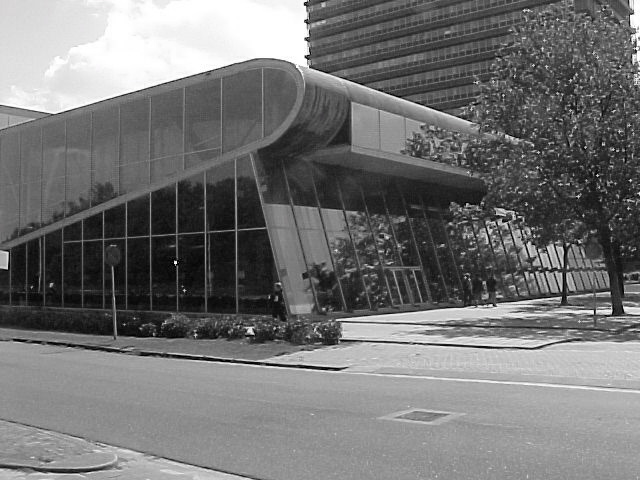
\includegraphics[width=0.3\textwidth,height=\textheight]{./tex2pdf.10928/2a53e7c630fc34751833a1c375097acbc5c345fb.jpg}
\caption{My caption}
\end{figure}

\end{frame}

\begin{frame}[fragile]{%
\protect\hypertarget{staged-builds}{%
Staged builds}}

This is quite easy

\pause

Just insert \texttt{.\ .\ .} on a new line when you want the slide to
appear incrementally.

\end{frame}

\begin{frame}[fragile]{%
\protect\hypertarget{code}{%
Code}}

You can use backticks to include inline code such as \texttt{x} or
\texttt{y}.

Use three backticks to introduce a code block:

\begin{verbatim}
main = print "Hello world!"
\end{verbatim}

\end{frame}

\begin{frame}[fragile]{%
\protect\hypertarget{syntax-highlighting}{%
Syntax highlighting}}

There are syntax highlighting options for the most widely used
languages.

\begin{Shaded}
\begin{Highlighting}[]
\NormalTok{foo y }\FunctionTok{=} \KeywordTok{let}\NormalTok{ x }\FunctionTok{=} \DecValTok{4} \KeywordTok{in}\NormalTok{ x }\FunctionTok{+}\NormalTok{ z}
  \KeywordTok{where}
\NormalTok{  z }\FunctionTok{=} \DecValTok{12}
\end{Highlighting}
\end{Shaded}

\end{frame}

\begin{frame}[fragile]{%
\protect\hypertarget{making-slides}{%
Making slides}}

I’ve included a Makefile to build slides.

You will need to have the Haskell tool \texttt{pandoc} installed:

\begin{verbatim}
> cabal install pandoc
> make
\end{verbatim}

\end{frame}

\begin{frame}{%
\protect\hypertarget{working-with-markdown}{%
Working with markdown}}

You may want to install the markdown mode for emacs (or some other
editor of choice).

I’ve included some file local variables at the bottom of this file – you
may find them useful.

\end{frame}

\begin{frame}{%
\protect\hypertarget{inline-latex}{%
Inline latex}}

You can always use \emph{inline} \LaTeX commands if you want.

But try to avoid this if you can.

Most Markdown commands should suffice.

\LaTeX is useful for formula’s

\begin{equation}
\tau + x = \sigma
\end{equation}

Or inline formulas, enclosed in dollar symbols like so \(\tau + x\).

\end{frame}

\begin{frame}{%
\protect\hypertarget{questions}{%
Questions}}

If you can’t get things to work, don’t hesitate to get in touch!

\end{frame}

\end{document}
